%!TEX root = main.tex
%In this section, we evaluate our proposed approach on synthetic as 
%well as real world examples.

We now show the practical performance of the dueling network.
We start with a simple policy evaluation task and then show larger scale results
for learning policies for general Atari game-playing.

%\begin{wrapfigure}{R}{6cm}
% \begin{figure}[t]
% 	\centering
% 	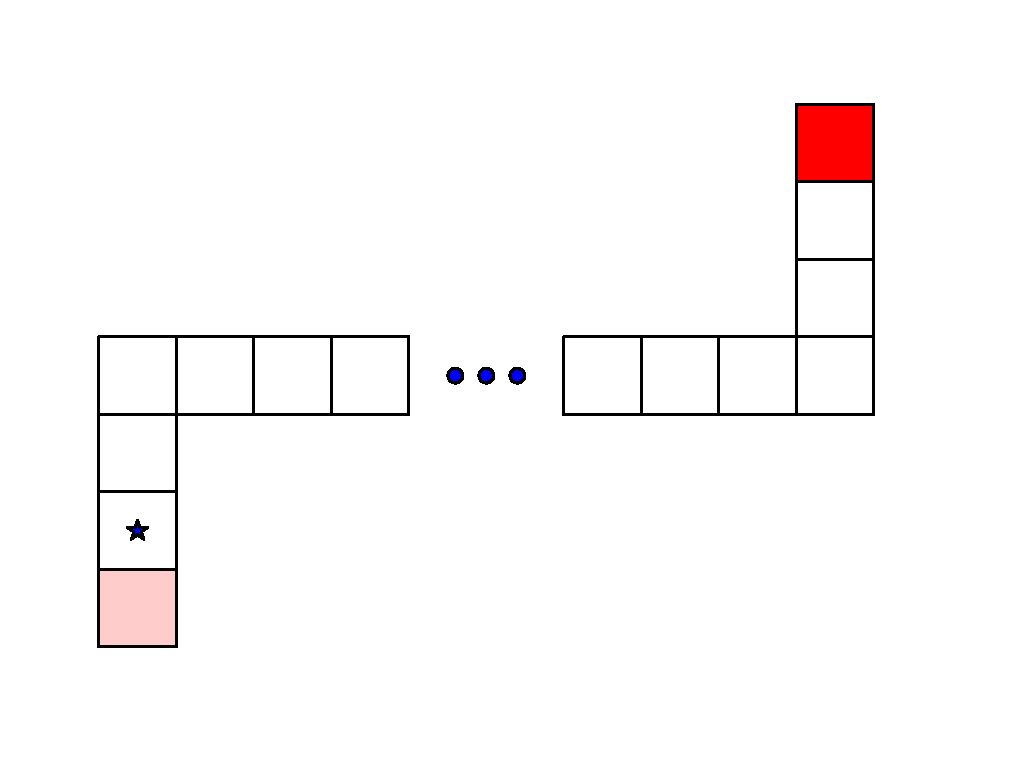
\includegraphics[scale=0.3]{./figs/corridor}
% 	\caption{The corridor environment. The star marks the starting state. 
% 		The redness of a state signifies the reward the agent receives upon arrival. 
% 		The game terminates upon reaching either reward state. 
% 		The agent's actions are going up, down, left, right and no action.
% 		\label{fig:corridor}}
% \end{figure}
%\end{wrapfigure}

\subsection{Policy evaluation}

\begin{figure*}[t]
\begin{center}
	\begin{tabular}{cccc}
		{\sc Corridor environment}& {\sc ~~~~~~5 actions} & {\sc 10 actions} & {\sc 20 actions} \\
		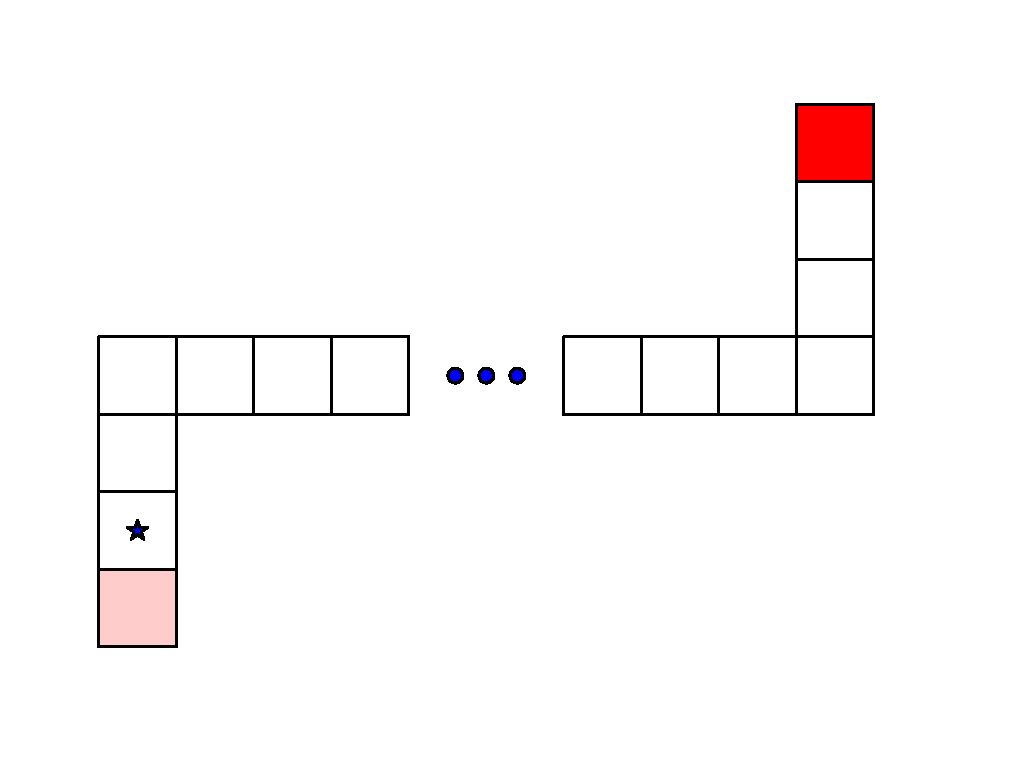
\includegraphics[scale=0.22]{./figs/corridor} &
		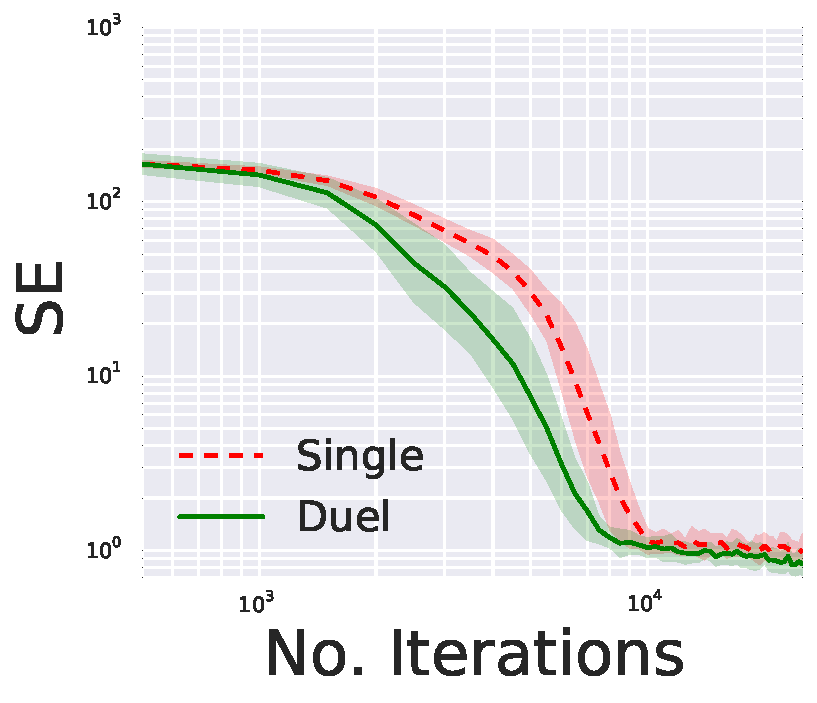
\includegraphics[scale=0.25]{./figs/duel_vs_Q_Q_5} &
		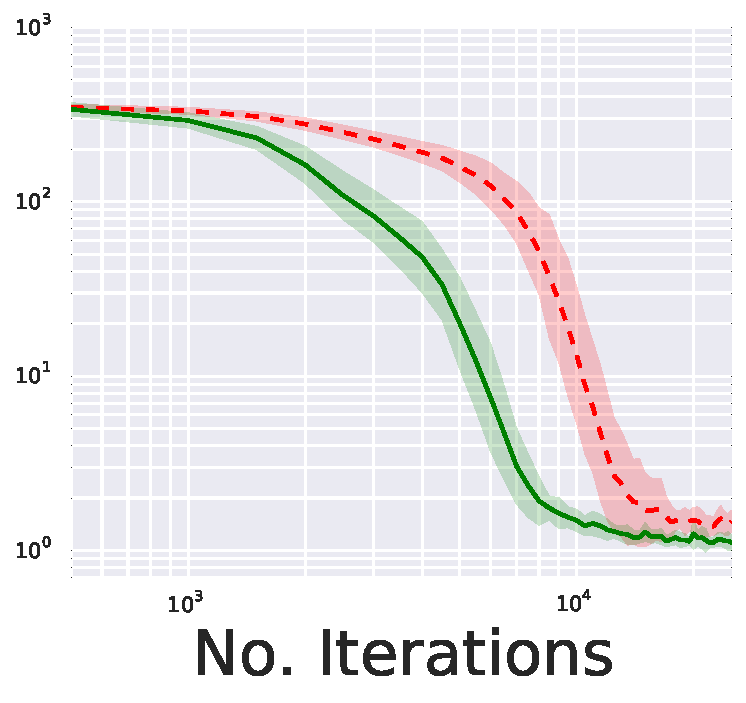
\includegraphics[scale=0.25]{./figs/duel_vs_Q_Q_10}&
		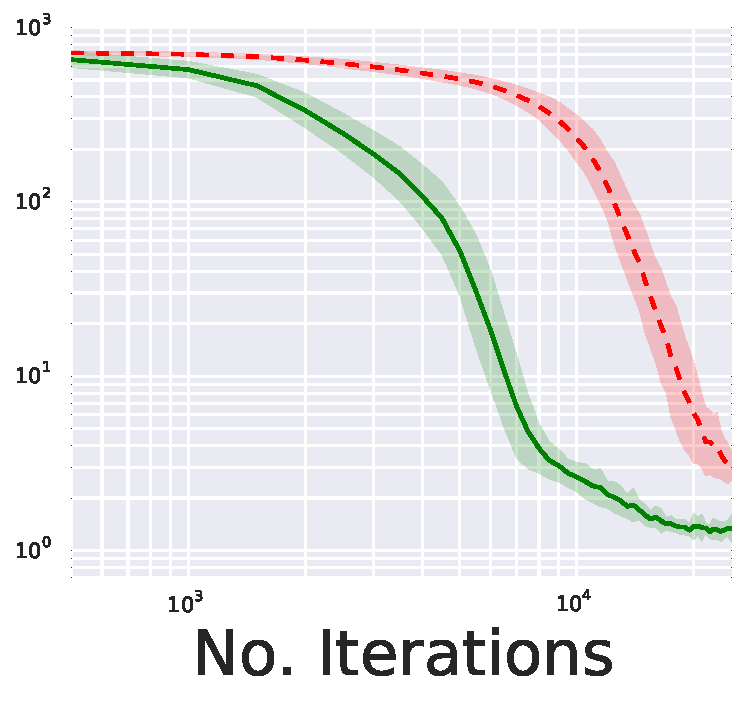
\includegraphics[scale=0.25]{./figs/duel_vs_Q_Q_20} \\
		{\bf (a)}& {\bf (b)} & {\bf (c)} & {\bf (d)} 
	\end{tabular}
	\vspace{-1em}
\end{center}
\caption{{\bf (a)} The corridor environment. The star marks the starting state. 
		The redness of a state signifies the reward the agent receives upon arrival. 
		The game terminates upon reaching either reward state. 
		The agent's actions are going up, down, left, right and no action.
Plots {\bf(b), (c)} and {\bf(d)} shows squared error for policy evaluation with 5, 10, and 20 actions on a log-log scale. The dueling network (Duel) consistently outperforms a conventional single-stream network (Single), with the performance gap increasing with the number of actions.
	\label{fig:corrResults}}
\end{figure*}


We start by measuring the performance of the dueling architecture on a policy evaluation task.
%Compared to control tasks, we argue that 
We choose this particular task because it is very useful for evaluating network architectures,
as it is devoid of confounding factors 
such as the choice of exploration strategy, and the interaction between policy improvement and
policy evaluation.


In this experiment, we employ temporal difference learning (without eligibility traces, \emph{i.e.}, $\lambda = 0$) to learn $Q$ values.
More specifically, given a behavior policy $\pi$, we seek to estimate
the state-action value $Q^{\pi}(\cdot, \cdot)$ by optimizing the sequence of costs of equation~(\ref{eq:loss}), with target
%$$
%L_i(\theta_i) = \E_{s,a \sim \mathcal{B}} \left\{ \left( y_i - Q(s,a; \theta_{i}) \right)^{2} \right\},
%$$
%where $\mathcal{B}(s,a)$ is a behaviour distribution over states and actions, and the target is
\begin{equation*}
y_i =  r +  \gamma  \E_{a' \sim \pi(s')}\left[ Q(s',a';\theta_i) \right]. 
\end{equation*}
The above update rule is the same as that of Expected SARSA~\cite{vanSeijen:2009}.
We, however, do not modify the behavior policy as in Expected SARSA.

To evaluate the learned $Q$ values, 
we choose a simple environment 
where the exact $Q^\pi(s,a)$ values can be computed separately for all $(s,a) \in \cal{S} \times \cal{A}$.
This environment, which we call the {\it corridor} is composed of three connected corridors.
A schematic drawing of the corridor environment is shown in Figure~\ref{fig:corrResults}, 
The agent starts from the bottom left corner of the environment and must move to the top right to get the largest reward.
A total of $5$ actions are available: go up, down, left, right and
no-op. We also have the freedom of adding an arbitrary number of no-op actions.
In our setup, the two vertical sections both have 10 states while the horizontal 
section has 50.


We use an $\epsilon$-greedy policy as the behavior policy $\pi$, which chooses a random action with probability $\epsilon$ or an action according to the optimal $Q$ function
$\argmax_{a \in \cal{A}}Q^*(s,a)$ with probability $1-\epsilon$. In our experiments, $\epsilon$ is chosen to be $0.001$.

We compare a single-stream $Q$ architecture with the dueling architecture
on three variants of the corridor environment with 5, 10 and 20 actions 
respectively. The 10 and 20 action variants are formed by adding no-ops 
to the original environment.
We measure performance by Squared Error (SE) against the 
true state values: $\sum_{s \in \mathcal{S}, a \in \mathcal{A}} ( Q(s,a;\theta) - Q^{\pi}(s, a) )^2$.
The single-stream architecture is a three layer MLP with $50$ units
on each hidden layer. 
The dueling architecture is also composed of three layers.
After the first hidden layer of 50 units, however, the network branches
off into two streams each of them a two layer MLP with 25 hidden units.
The results of the comparison are summarized in Figure~\ref{fig:corrResults}.

The results show that with $5$ actions, both architectures converge at about the same speed.
However, when we increase the number of actions, the dueling
architecture performs better than the traditional $Q$-network. In the dueling network,
the stream ${V}(s;\theta,\beta)$ learns a
general value that is shared across many similar actions at $s$, hence leading to faster convergence. This is a very promising result because many control tasks with large action spaces have this property, and consequently we should expect that the dueling network will often lead to much faster convergence than a traditional single stream network. In the following section, we will indeed see that the dueling network results in substantial gains in performance in a wide-range of Atari games.

%which is a common
%occurrence in many control tasks.


\subsection{General Atari Game-Playing}

We perform a comprehensive evaluation of our proposed method on the Arcade Learning Environment~\cite{Bellemare:2013},
which is composed of 57 Atari games. The challenge is to deploy a single algorithm and architecture,
with a fixed set of hyper-parameters, to learn to play all the games
given only raw pixel observations and game rewards. 
This environment is very demanding because it is both comprised of a large number of highly diverse games and the observations are high-dimensional.

We follow closely the setup of~\citet{vanHasselt:2015} and compare
to their results using single-stream $Q$-networks. We train the dueling network with the DDQN algorithm as presented in Appendix~\ref{sec:ddqn_alg}. At the end of this section, we incorporate
prioritized experience replay~\cite{Schaul:2015}.


Our network architecture has the same low-level convolutional structure of DQN~\cite{Mnih:2015,vanHasselt:2015}.
There are 3 convolutional layers followed by 2 fully-connected layers. The first convolutional layer has 32 $8 \times 8$ filters with stride 4, the second 64 $4 \times 4$ filters with stride 2, and the third and final convolutional layer consists 64 $3 \times 3$ filters with stride 1. 
As shown in Figure~\ref{fig:duelnet},
the dueling network splits into two streams of fully connected layers. 
The value and advantage streams both have a fully-connected layer with 512 units. 
The final hidden layers of the value and advantage streams are both fully-connected
with the value stream having one output and the advantage as many outputs
as there are valid actions\footnote{The number of actions ranges between 3-18 actions in the ALE environment.}.
We combine the value and advantage streams using the module described by Equation~(\ref{eq:combo2}).
Rectifier non-linearities \cite{Fukushima:1980} are inserted between all adjacent layers.

%We refer to the popular convolutional Q-network
%architectures used in~\citet{Mnih:2015,vanHasselt:2015,Schaul:2015} as single stream networks.

We adopt the optimizers and hyper-parameters of~\citet{vanHasselt:2015},
with the exception of the learning rate which we chose to be slightly lower (we do not do this for double DQN as it can deteriorate its performance).
Since both the advantage and the value stream propagate gradients to the 
last convolutional layer in the backward pass, we rescale the combined gradient
entering the last convolutional layer by $1/\sqrt{2}$. This simple heuristic mildly increases stability.
In addition, we clip the gradients to have their norm less than or equal to 10. This clipping is not standard practice in deep RL, but common in recurrent network training \cite{Bengio:2013}. 

To isolate the contributions of the dueling architecture, we re-train DDQN
with a single stream network using exactly the same procedure 
as described above. Specifically, we apply gradient clipping, and
use $1024$ hidden units for the first fully-connected layer of the
network so that both architectures (dueling and single) have roughly the same
number of parameters. We refer to this re-trained model as \emph{Single Clip}, while the original trained model of~\citet{vanHasselt:2015} is referred to as \emph{Single}.

% During training, if the network produces outputs $\mathbf{o} = Q(s, \cdot;\theta,\alpha,\beta), \forall a \in \cal{A}$ for input $s$
% and we have associated targets $\mathbf{y}$ and
% $g = \nabla_{\theta,\alpha,\beta} Q(s,a;\theta,\alpha,\beta)$, then if $n = || g(s,\mathbf{o},\mathbf{y}) ||_2 \ge 10$ we instead use $g' = \frac{10g}{n}$.
% Gradient clipping, although not a commonly adopted practice
% for training convolutional networks, helps in the context of $Q$ learning.

% All three architectures are trained with the same hyper-parameters.
% As shown in Figure~\ref{fig:trainCurves}, 
% gradient clipping clearly helps with training. 
% The dueling architecture still maintains
% a very significant advantage over the traditional $Q$ architecture 
% in the presence of gradient clipping.
% Overall, the dueling architecture does equally or better on 75.4\% of the games (43 out of 57). 

\begin{figure}[t!]
\begin{center}
	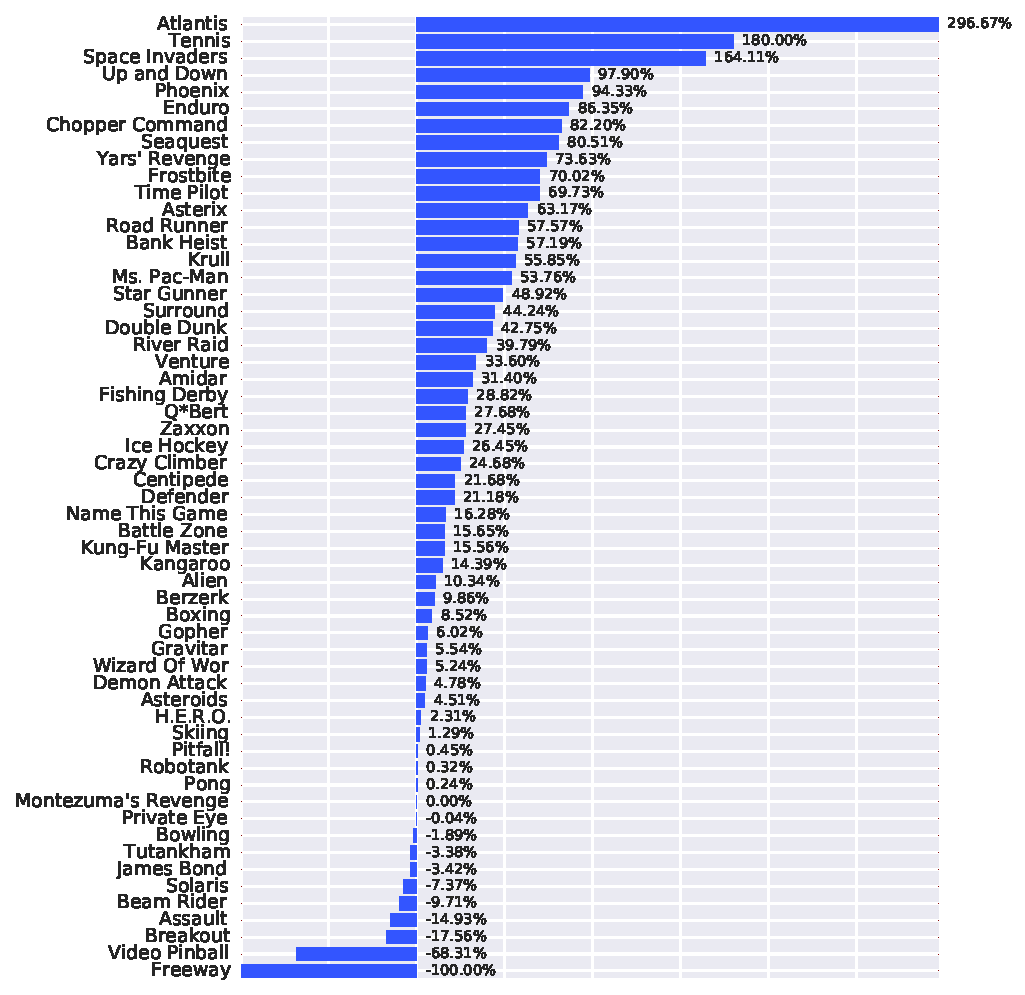
\includegraphics[scale=0.47]{./figs/DG05_vs_DQBa}
\end{center}
\caption{\label{fig:at30} Improvements of dueling architecture over the baseline Single network of~\citet{vanHasselt:2015}, using the metric described in Equation~(\ref{eq:metric}). Bars to the right indicate by how much the dueling network outperforms the single-stream network.}
\end{figure}
%\begin{wrapfigure}{R}{5cm}
%\vspace{-30pt}

%\end{wrapfigure}

As in~\cite{vanHasselt:2015}, 
we start the game with up to \emph{30 no-op} actions to provide random starting positions for the agent.
To evaluate our approach, we measure improvement in percentage (positive or negative) 
in score over the better of human and baseline agent scores: 
\be
\label{eq:metric}
{\footnotesize
\frac{\mbox{\small Score}_{\mbox{\tiny Agent}} - \mbox{\small Score}_{\mbox{\tiny Baseline}}}
	{\small
		\max\{
			\mbox{Score}_{\mbox{\tiny Human}}, \mbox{Score}_{\mbox{\tiny Baseline}} 
		 \}
	-  \mbox{Score}_{\mbox{\tiny Random}}
	}.
}
\ee
We took the maximum over human and baseline agent scores as it prevents insignificant 
changes to appear as large improvements 
when neither the agent in question nor the baseline are doing well.
For example, an agent that achieves 2\% human performance should not be interpreted 
as two times better when the baseline agent achieves 1\% human performance.
We also chose not to measure performance in terms of percentage of human performance alone
because a tiny difference relative to the baseline on some games can translate into hundreds of
percent in human performance difference.


The results for the wide suite of 57 games are summarized in~Table~\ref{tb:result}. Detailed results are presented in the Appendix.

Using this 30 no-ops performance measure, it is clear that the dueling network (Duel Clip) does substantially better than the Single Clip network of similar capacity. It also does considerably better than the baseline (Single) of~\citet{vanHasselt:2015}. For comparison we also show results for the deep $Q$-network of \citet{Mnih:2015}, referred to as Nature DQN.






Figure~\ref{fig:at30} shows the improvement of the dueling network over the baseline Single network of~\citet{vanHasselt:2015}. Again, we seen that the improvements are often very dramatic.


As shown in Table~\ref{tb:result}, Single Clip performs better than Single. We verified that this gain was mostly brought in by gradient clipping. For this reason, we incorporate gradient clipping in all the new approaches.  





%\footnote{	When calculating the human performance percentage for the game	Video Pinball, the random scores are set to zero. 	This is because human scores 	on this game are lower than that of a random agent making the calculation of	human performance percentage invalid.	Resetting the random score does not affect the median scores of the agents	considered. The mean scores, however, are affected.}

\begin{table}[t]
\caption{Mean and median scores across all 57 Atari games, measured in percentages of human performance.}
\label{tb:result}
\small
\begin{center}
\begin{tabular}{l|rr|rr}
\multicolumn{1}{c}{\bf }  &\multicolumn{2}{c}{\bf 30 no-ops} &\multicolumn{2}{c}{\bf Human Starts} \\
 \hline
\multicolumn{1}{c}{\bf }  &\multicolumn{1}{r}{\bf Mean} &\multicolumn{1}{r}{\bf Median}&\multicolumn{1}{r}{\bf Mean} &\multicolumn{1}{r}{\bf Median}
\\ \hline 
Prior. Duel Clip  &  {\bf 591.9}\%  & {\bf 172.1}\% &  {\bf 567.0}\%  & {\bf 115.3}\% \\
Prior. Single&  434.6\%  & 123.7\% &  386.7\%  & 112.9\% \\
\hline
Duel Clip       &  {\bf 373.1}\%  & {\bf 151.5}\% &  {\bf 343.8}\%  & {\bf 117.1}\% \\
Single Clip  &  341.2\%  & 132.6\% &  302.8\%  & 114.1\% \\
Single            &  307.3\%   & 117.8\% &  332.9\%   & 110.9\% \\
\hline
Nature DQN            &  227.9\%   & 79.1\% &  219.6\%   & 68.5\% 
\end{tabular}
\end{center}
\end{table}

Duel Clip does better than Single Clip 
on 75.4\% of the games (43 out of 57). It also achieves higher scores compared to the Single baseline on 80.7\% ($46$
out of $57$) of the games. Of all the games with $18$ actions, 
Duel Clip is better $86.6$\% of the time (26 out of 30).
This is consistent with the findings of the previous section.
Overall, our agent (Duel Clip) achieves human level performance on 42 out of 57 games.
Raw scores for all the games, as well as measurements in human performance percentage,
are presented in the Appendix.
% In Figure~\ref{fig:natureComp}, we show a comparison between our
% agent, DQN~\cite{mnih2015human}, and human expert.





% A few training curves, shown in Figure~\ref{fig:trainCurves}, 
% compare the dueling architecture, and DDQN with the traditional $Q$ architecture with
% and without gradient clipping.
% \begin{figure}[h]
% \begin{center}
% 	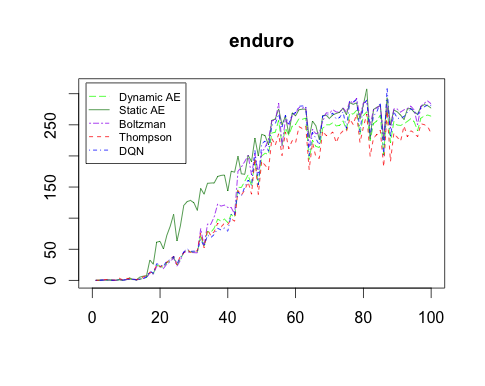
\includegraphics[scale=0.19]{./figs/enduro}
% 	\includegraphics[scale=0.19]{./figs/kung_fu_master}
% 	\includegraphics[scale=0.19]{./figs/riverraid} 
% 	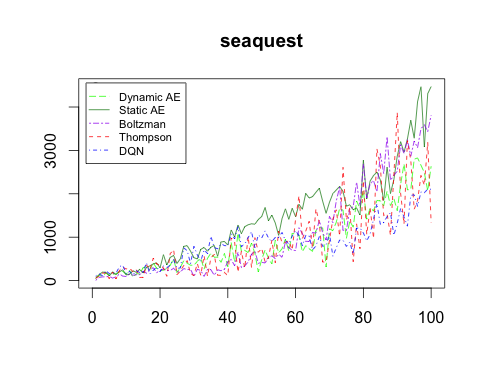
\includegraphics[scale=0.19]{./figs/seaquest}
% \end{center}
% \caption{Performance evaluated at training time on four Atari games. The curves correspond to three instances of the DDQN algorithm using a convolutional network of similar size to the dueling network (Q net) using the same convolutional network and gradient clipping (Q net Clip) and using the dueling network (Duel).  
% 	\label{fig:trainCurves}}
% \end{figure}
% Seaquest $0.039$ $0.039$
% Ms. Pacman $0.032$ $0.042$


% \subsubsection*{Human Random Starts}
{\bf Robustness to human starts.}
One shortcoming of the 30 no-ops metric is that an agent does not necessarily have
to generalize well to play the Atari games.
Due to the deterministic nature of the Atari environment, 
from an unique starting point, an agent could learn to achieve good performance by simply 
remembering sequences of actions.

To obtain a more robust measure, we adopt the methodology of 
~\citet{Nair:2015}.
Specifically, for each game, we use 100 starting points sampled from a human expert's trajectory.
From each of these points, an evaluation episode is launched for up to 108,000 frames.
The agents are evaluated only on rewards accrued after the starting point. We refer to this metric as \emph{Human Starts}.

As shown in Table~\ref{tb:result}, under the Human Starts metric, Duel Clip once again outperforms the single stream variants. In particular, our agent does better than the Single baseline on 70.2\% (40 out of 57) games
and on games of $18$ actions, Duel Clip is 83.3\% better (25 out of 30).



\begin{figure}[t!]
\begin{center}
	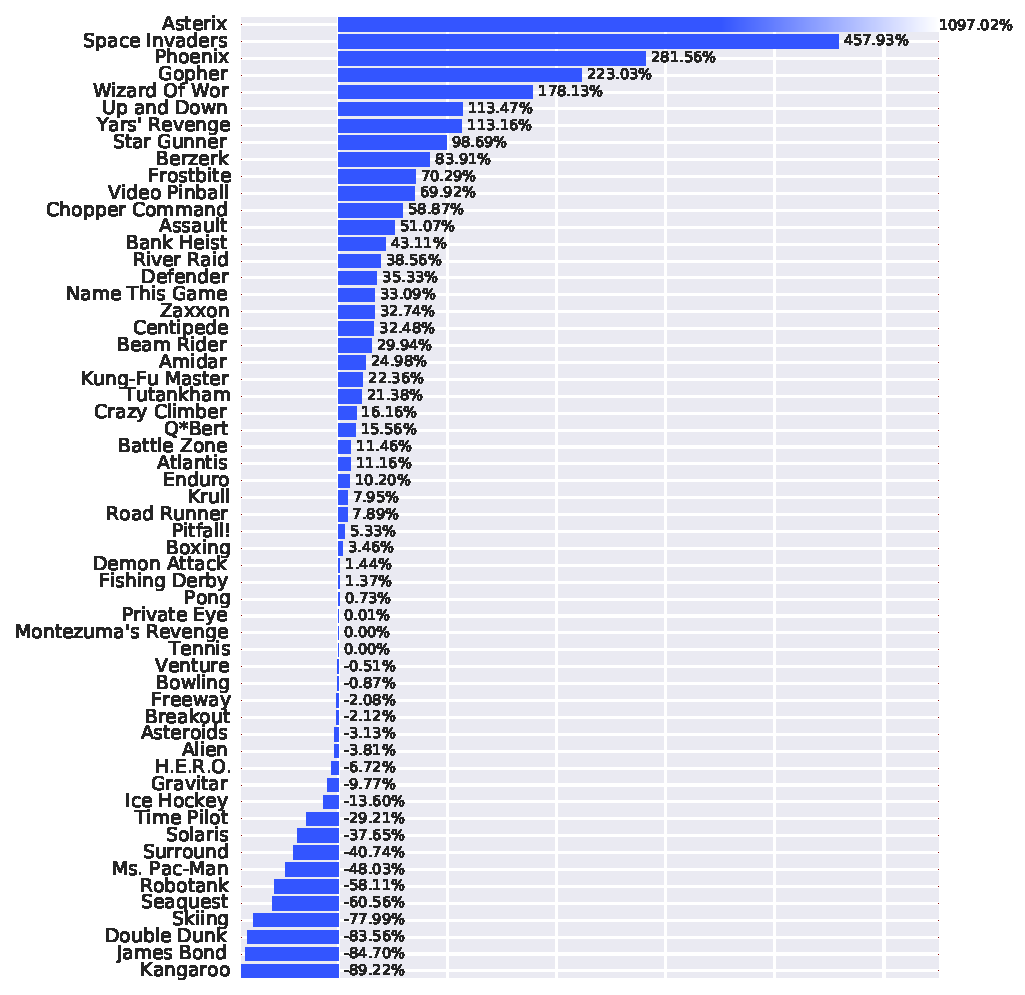
\includegraphics[scale=0.47]{./figs/pri_duel_vs_pri_11c}
\end{center}
\caption{\label{fig:at30_priduel} 
Improvements of dueling architecture over Prioritized DDQN baseline, using the same metric as Figure~\ref{fig:at30}. 
Again, the dueling architecture leads to significant improvements over the single-stream baseline on the majority of games.
}
\end{figure}


{\bf Combining with Prioritized Experience Replay.}
\label{sec:prioritizedduel}
The dueling architecture can be easily combined with other algorithmic improvements. 
In particular, prioritization of the experience replay has been shown to significantly improve performance of Atari games~\cite{Schaul:2015}. 
Furthermore, as prioritization and the dueling architecture address very different aspects of the learning process, their combination is promising. 
So in our final experiment, we investigate the integration of the dueling architecture with prioritized experience replay.
We use the prioritized variant of DDQN (Prior. Single) as the new baseline algorithm, which replaces with the uniform sampling
of the experience tuples by rank-based prioritized sampling. 
We keep all the parameters of the prioritized replay as described in~\cite{Schaul:2015}, namely
a priority exponent of $0.7$, and an annealing schedule on the importance sampling exponent from $0.5$ to $1$.
% , as well as sorting the heap every $10^6$ frames. %TODO
We combine this baseline with our dueling architecture (as above), and again use gradient clipping (Prior. Duel Clip).

Note that, although orthogonal in their objectives, these extensions (prioritization, dueling and gradient clipping) interact in subtle ways. 
For example, prioritization interacts with gradient clipping, as sampling transitions with high absolute TD-errors more often leads to gradients with higher norms. 
To avoid adverse interactions, we roughly re-tuned the learning rate and the gradient clipping norm on a subset of $9$ games. As a result of rough tuning, we settled on $6.25 \times 10^{-5}$ for the learning rate and $10$ for the gradient clipping norm (the same as in the previous section).

When evaluated on all $57$ Atari games, our prioritized dueling agent performs significantly better than both the prioritized baseline agent and the dueling agent alone.
The full mean and median performance against the human performance percentage is shown in Table~\ref{tb:result}. When initializing the games using up to 30 no-ops action, we observe mean and median scores of 591\% and 172\% respectively.
The direct comparison between the prioritized baseline and prioritized dueling versions, using the metric described in Equation~\ref{eq:metric}, is presented in Figure~\ref{fig:at30_priduel}.

The combination of prioritized replay and the dueling network results in vast improvements over the previous state-of-the-art in the popular ALE benchmark.




% When initializing the games using up to 30 no-ops, we observed 591\% mean, and 172\% median, normalized scores. This agent also achieves the best reported performance on 6 Atari games (of which 5 were not in the set of games used for tuning). 


% subsection  (end)



{\bf Saliency maps.} To better understand the roles of the value
and the advantage streams, we compute saliency maps~\cite{Simonyan:2013}.
More specifically, to visualize the salient part of the image as seen by the value stream,
we compute the absolute value of the Jacobian of $\widehat{V}$ with respect to the input frames:
$|\nabla_{s} \widehat{V}(s ;\theta)|.$
Similarly, to visualize the salient part of the image as seen by the advantage stream,
we compute $|\nabla_{s} \widehat{A}(s, \argmax_{a'} \widehat{A}(s, a');\theta)|$.
Both quantities are of the same dimensionality as the input frames and therefore
can be visualized easily alongside the input frames.

Here, we place the gray scale input frames in the green and blue channel and
the saliency maps in the red channel.
All three channels together form an RGB image.
Figure~\ref{fig:saliency} depicts the
value and advantage saliency maps on the Enduro game for two different time steps. 
As observed in the introduction, the value stream pays attention 
to the horizon where the appearance of a car could affect future performance.
The value stream also pays attention to the score.
The advantage stream, on the other hand, cares more about cars 
that are on an immediate collision course.




